%% TIKZ DRAWING OF CALIFES ELEMENTS
%% TO BE INCLUDED INTO A LATEX DOCUMENT
%% K. Sjobak, 2018

\begin{tikzpicture}
    
    \solRect{-3.5}{0.5}{-3.2}{0.7};
    \solRect{-3.5}{-0.5}{-3.2}{-0.7};
    \draw[->,ultra thick] (-3.2,0)--(-3.8,0);
    \node[align=left,anchor=west] at (-3.2,0) {Solenoid};

    \kickerHV[0]{-1.5}{}{1}{blue};
    \node[align=left,anchor=west] at (-1.3,0) {Dipole};

    \correctorMagnet{0.0}{};
    \node[align=left,anchor=west] at (0.2,0) {Corrector\\ magnet};
    
    \lensF{2.0}{};
    \lensD{2.5}{};
    \node[align=left,anchor=west] at (2.75,0) {Focusing /\\ defocusing\\ magnet};

    \BTV[0.5]{5}{};
    \node[align=left,anchor=west] at (5.3,0.5) {BTV screen};
    
    \cBPM[-0.05]{5}{};
    \node[align=left,anchor=west] at (5.3,-0.05) {Cavity BPM};
    
    \iBPM[-0.5]{5}{};
    \node[align=left,anchor=west] at (5.3,-0.5) {Inductive BPM};

\end{tikzpicture}

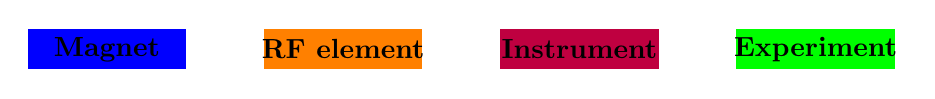
\begin{tikzpicture}

    \filldraw[blue] (-2,-1.5) rectangle (0,-1.);
    \node at (-1,-1.25) {\textbf{Magnet}};

    \filldraw[orange] (1,-1.5) rectangle (3,-1.);
    \node at (2,-1.25) {\textbf{RF element}};

    \filldraw[purple] (4,-1.5) rectangle (6,-1.);
    \node at (5,-1.25) {\textbf{Instrument}};

    \filldraw[green] (7,-1.5) rectangle (9,-1.);
    \node at (8,-1.25) {\textbf{Experiment}};

\end{tikzpicture}